\chapter{Modelo de Red de Caspasas}
\label{cap:modelo}

Actualmente, en biología de sistemas se utilizan los modelos matemáticos de bioquímica con el objetivo de modelar redes de proteínas y reacciones que ocurren \ening{in vivo}. Es así que se utilizan redes de ecuaciones diferenciales ordinarias que surgen de la ley de acción de masas\cite{Chen2010}. Estos modelos son validados mediante contraste experimental y poseen valor predictivo a la hora de estudiar un sistema o diseñar nuevos experimentos.

%sirven, también, para explicar la aproximación de Michaelis Menten. En este caso, las ecuaciones diferenciales ordinarias

Es de conocimiento general los modelos de Michaelis y Menten (1913) desarrollados hace aproximadamente un siglo para comprender la dinámica enzimática. Este a su vez se basaba en los hallazgos de Haldi (1902) y fue clarificado posteriormente por Briggs y Haldane (1925) una década después. Luego fueron extendidos en las décadas subsiguientes por Monod et. al (1965), Koshland (1966) y Goldbeter y Koshland (1981). Estos modelos se concentran en describir reacciones enzimáticas controladas \ening{in vitro} y en condiciones de concentraciones homogéneas\cite{Chen2010}. Extensiones de los mismos son utilizadas para modelar cascadas de señalización más complejas en las células.


%%%%%%%%%%%%%%%%%%%%%%%%%%%%%%%%%%%%%%%%%%%%%%%%%%%
\section{Ley de acción de masas}

La ley fundamental de una reacción química es la de acción de masas. Esta describe la tasa a la cual los elementos químicos, sean tanto macromoléculas o simples iones, colisionan e interactúan para formar los distintos productos. Comencemos por considerar una reacción simple en la que los sustratos $A$ y $B$ colisionan para formar $C$, es decir,

\begin{center}
\ce{A + B ->[k] C,}
\end{center}

\noindent donde $k$ se denomina la constante de reacción. Esta surge de considerar que las colisiones de las moléculas en el sistema en equilibrio térmico se dan de forma completamente aleatoria. Esta constante depende a su vez de la relación entre los tamaños de las especies involucradas, su geometría y otros parámetros que pueden reducirse a la probabilidad de encuentro y reacción exitosa\cite{Gillespie1977}.

Asumiendo que la concentración de las especies en estudio pueden ser descriptas mediante funciones continuas, y que cada una de sus reacciones químicas pueden representarse como procesos continuos, es posible construir una serie de ecuaciones diferenciales acopladas que describan la dinámica. En este caso particular, la variación de la concentración del producto ($C$) que descripta por\cite{Gillespie1977}

\begin{equation}
    \frac{dC}{dt} = k[A][B],
\end{equation}

\noindent donde $[A]$ y $[B]$ se refieren a las concentraciones de $A$ y $B$ respectivamente. Al igual que la ley de Ohm o la ley de Newton para enfriamiento, esta tiene cierto rango de validez. En primer lugar, si se trabaja a concentraciones altas, duplicar la concentración no implica que necesariamente se duplique la tasa de formación de producto. En el otro extremo, si se utilizan concentraciones muy bajas, puede que representar la concentración como una variable continua no sea la mejor opción\cite{Keener1998}.

A continuación, si deseamos estudiar que sucede con reacciones reversibles podemos utilizar la misma metodología, en particular, si analizamos la siguiente reacción

\begin{center}
\ce{A + B <=>[$k_+$][$k_-$] C,}
\end{center}

\noindent podemos describir la tasa de consumo y producción de $A$ como

\begin{equation}
    \frac{dA}{dt} = -k_+ [A][B] + k_- [C],
\end{equation}

\noindent donde se debe prestar especial atención a los signos de cada término ya que determinan si se trata de producción o consumo de la especie en cuestión. Podemos estudiar la condición de equilibrio del sistema, que debe ser interpretada como que las tasas de asociación y disociación son las mismas, obteniéndose una concentración constante de cada especie. Usando entonces que $[C]_{eq} = \frac{k_+}{k_-} [A]_{eq} [B]_{eq}$ y que $[A]+[C] = A_0$ es constante ya que no hay otras reacciones que los involucren, llegamos a

\begin{equation}
    [C] = A_0 \frac{[B]}{K_{eq} + [B]},
\end{equation}

\noindent donde $K_{eq} = k_+/k_-$ es la constante de equilibrio y da cuenta de la preferencia del sistema para estar en el estado asociado por sobre el disociado\cite{Keener1998}.


%%%%%%%%%%%%%%%%%%%%%%%%%%%%%%%%%%%%%%%%%%%%%%%%%%%
\section{Cinética Enzimática}
\label{sec:CineticaEnzimatica}
Las enzimas son catalizadores, en general proteínas, que colaboran en la conversión de sustratos en producto, manteniéndose inalteradas una vez terminada la reacción. Entre sus características más importantes encontramos su elevado poder catalítico, su especificidad y la posibilidad de regularlas. Estas son especialmente eficientes para acelerar reacciones biológicas, aumentando hasta 10 millones de veces la velocidad de reacción. Típicamente se encuentran reguladas por una complicada red de lazos de retroalimentación, tanto positivos como negativos, permitiendo un control preciso sobre la tasa de reacción\cite{Keener1998}.

Un modelo para describir esta cinética fue propuesto por Michaelis y Menten. En el esquema de la reacción, la enzima ($E$) convierte al sustrato ($S$) en producto ($P$) en un proceso de dos pasos. En el primer paso, se unen la enzima y el sustrato formando un complejo enzima-sustrato ($C$); para luego dar lugar a la formación del producto y la liberación de la enzima. Esta reacción puede representarse como

\begin{center}
\ce{S + E <=>[$k_+$][$k_-$] C ->[$k_c$] P.}
\end{center}

\noindent Aunque en general el producto puede volver a unirse a la enzima, y estas aceleran las reacciones en ambos sentidos, las condiciones en que se estudian estas reacciones son tales que el producto es removido constantemente, lo que previene la reacción inversa.

Analicemos las ecuaciones diferenciales que surgen al aplicar ley de acción de masas en este sistema

\begin{align}
    \frac{ds}{dt} =& k_- c - k_+ se \label{eq:cin_sens}\\
    \frac{de}{dt} =& (k_- + k_c) c - k_+ se\\
    \frac{dc}{dt} =& k_+ se - (k_- + k_c) c\\
    \frac{dp}{dt} =& k_c c, \label{eq:cin_prod}\\
\end{align}

\noindent donde se uso que $[E]=e$, $[S]=s$, $[C]=c$ y $[P]=p$. Podemos apreciar que $\frac{de}{dt} + \frac{dc}{dt} = 0$, que corresponde a la existencia de una cantidad conservada, en este caso la enzima. Esto se condice con lo explicado previamente ya que la enzima acelera la reacción, pero se mantiene inalterada una vez culminada la reacción. De aquí que $e+c=e_0$ donde $e_0$ es la cantidad de enzima disponible. Por otro lado, también se aprecia que $\frac{ds}{dt} + \frac{dc}{dt} + \frac{dp}{dt} = 0$, que, dado que no hay síntesis de sustrato ni degradación de producto incluídas hasta ahora, se conserva la cantidad de sustrato más producto en todos sus estados.


%%%%%%%%%%%%%%%%%%%%%%%%%%%%%%%%%%%%%%%%%%%%%%%%%%%
\section{Modelo de Red de Caspasas}

Con el objetivo de modelar el sistema biológico en estudio, se buscó en la bibliografía modelos basados en ecuaciones diferenciales acopladas construidas a partir de ley de acción de masas que se apliquen a la red de caspasas en estudio. \textit{Sorger et al.} dedicaron mucho esfuerzo a construir y entrenar un modelo matemático que describa correctamente la cascada de caspasas. Dicho modelo cuenta con 58 especies que corresponden a 18 moléculas cuyas condiciones iniciales son distintas de 0 y 40 especies adicionales que representan complejos, proteínas clivadas, o formas localizadas de especies iniciales que interactúan mediante 28 reacciones con 70 constantes de reacción que son no nulas\cite{Sorger2008}.

\begin{figure}
    \centering
    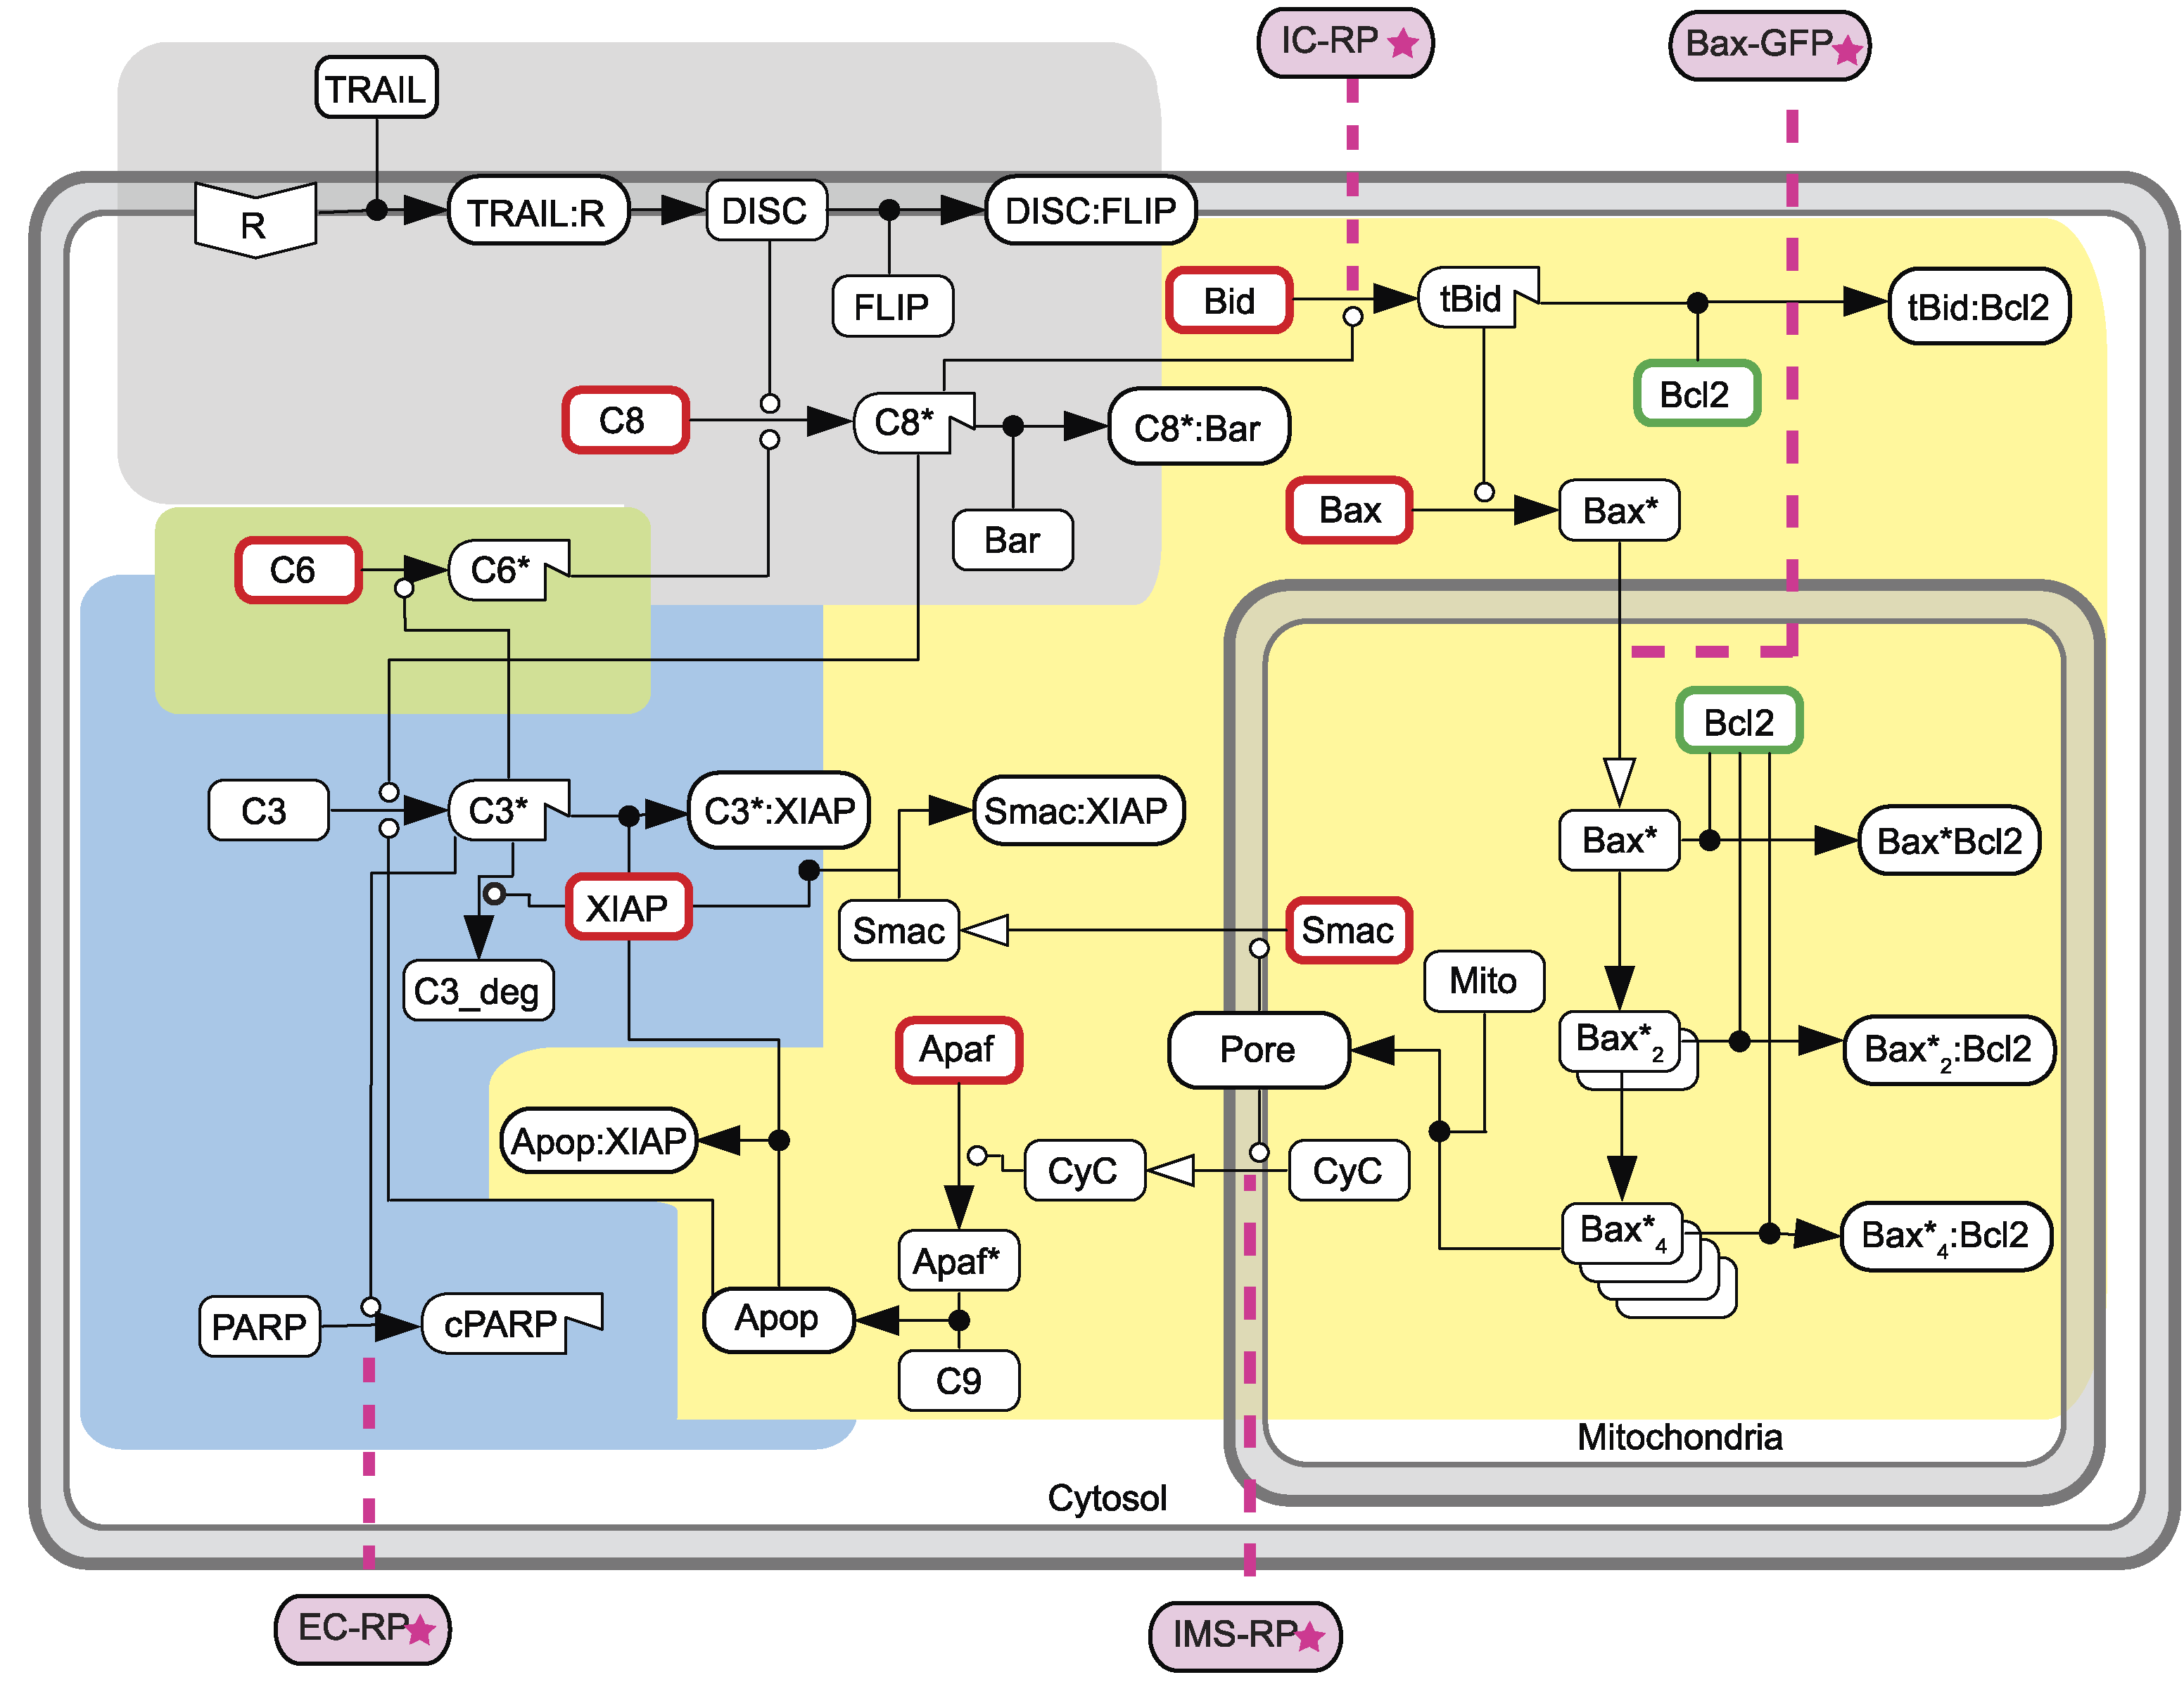
\includegraphics[width=0.9\textwidth]{./img/Cap3/ModeloCompleto.png}
    \caption{Esquema representativo de las reacciones modeladas por \textit{Sorger et al.} mediante ecuaciones diferenciales acopladas. Todas las especies que juegan un papel importante en la cascada de señalización caspasas se encuentran incluidas\cite{Albeck2008}.}
    \label{fig:ModeloCompleto}
\end{figure}

Como se muestra en la figura \ref{fig:ModeloCompleto}, el modelo puede dividirse en cuatro subcircuitos. El primero (gris) consiste en una representación agrupada de la unión del factor de necrosis tumoral (\ening{TNF} por sus siglas en inglés) o ligando de inducción de apoptosis relacionado con TNF (\ening{TRAIL} por sus siglas en inglés) al receptor y la subsecuente activación de la procaspasa-8 mediante el complejo de señalización de inducción de muerte (\ening{DISC} por sus siglas en inglés) unido al receptor. En segundo lugar (azul), se muestra la cascada enzimática en que la caspasa-8 activa cliva a la procaspasa-3, la cual a su vez cliva otros sustratos efectores. Por otro lado, se muestra la vía mitocondrial (amarillo) por la cual la caspasa-8 activa cliva a Bid para dar lugar a la activación de Bax que luego dara lugar a la formación de poros en la membrana mitocondrial por los cuales citocromo C (\ening{CyC} por sus siglas en inglés) y Smac son traslocados al citosol; una vez ahí, se forma el apoptosoma a partir de Apaf-1 y procaspasa-9, para clivar y activar aún más moléculas de caspasa-3. Por último, se representa (verde) un lazo de retroalimentación positivo entre la caspasa-3 y la procaspasa-8 mediado por la caspasa-6, que es clivada y activada por la caspasa-3\cite{Sorger2008}.

Sumado a las aproximaciones implícitas en ley de acción de masas, la construcción de este modelo agrega otras tres aproximaciones que deben tenerse en cuenta. En primer lugar, la formación de DISC y el apoptosoma que incluyen unión de varias proteínas fue simplificado usando una representación con parámetros agrupados. En segundo lugar, se omitió la síntesis de cualquier proteína. Por último, especies con actividades similares fueron representadas por una única especie, entre ellas están: caspasa-8 y caspasa-10, caspasa-3 y caspasa-7 y la familia de proteínas similares a Bcl-2\cite{Sorger2008}.

El modelo matemático diseñado por \textit{Sorger et al.} fue entrenado con datos experimentales que provienen de experimentos de microscopía de células vivas, citometría de flujo e inmunoblotting de células perturbadas con depleción de proteínas o sobreexpresión. El modelo fue entrenado para describir adecuadamente el comportamiento de células normales y perturbadas ante estímulos con TRAIL\cite{Sorger2008}.

El modelo desarrollado por \textit{Sorger et al.} se encuentra libre para descargar e implementar en \textit{MatLab}. Se descargó dicho modelo y se adaptó para que describa el comportamiento de las especies correspondientes al sensor utilizado. Para ello fue necesario, en primer lugar, probar el algoritmo para reproducir algunas de las imágenes de la publicación y comprender los efectos que producen las variaciones de distintos parámetros.


%%%%%%%%%%%%%%%%%%%%%%%%%%%%%%%%%%%%%%%%%%%%%%%%%%%
\section{Adaptación del Modelo}

Considerando que se desea evaluar la actividad de las tres vías de caspasas descriptas en la Introducción se adicionaron al sistema modelado tres sensores que son clivados por las caspasas-3, -8 y -9, para estudiar las vías efectora, extrínseca e intrínseca, respectivamente. Se añadieron tres especies distintas para cada sensor, a saber, el sensor sin clivar en estado dimérico, el sensor formando complejo con la caspasa y el sensor clivado en estado monomérico. Las constantes de unión, disociación y formación de producto se eligieron iguales a las correspondientes a las distintas caspasas ya que se asume que trabajan por igual sobre cualquiera de los distintos sustratos.

\begin{figure}
    \centering
    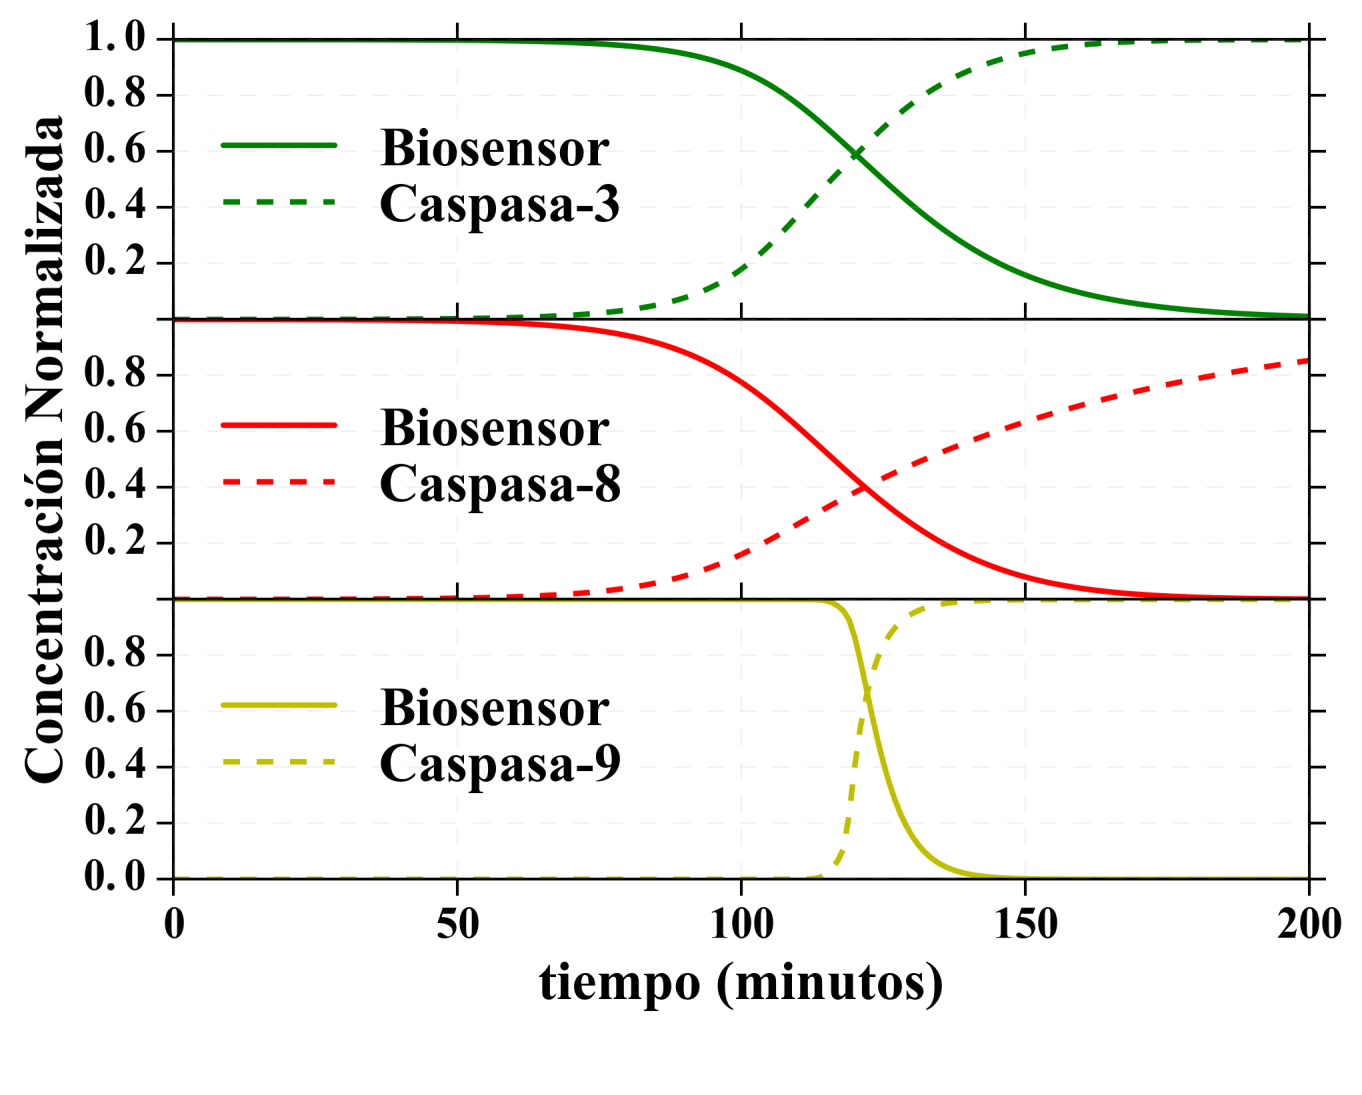
\includegraphics[width=0.65\textwidth]{./img/Cap3/AdicSensores.png}
    \caption{Se graficaron las concentraciones relativas de las tres caspasas de interés superpuestas con las correspondientes a los sensores adicionales del sistema biológico.}
    \label{fig:AdicSensores}
\end{figure}

Se asumió como hipótesis que los sensores sintetizados por la célula se producen en estado dimérico y estos son clivados únicamente por la caspasa activa de la célula durante la cascada de señalización. Por esta razón, se seleccionaron las condiciones iniciales de los sensores de forma tal que las concentraciones de las especies correspondientes al sensor clivado y en complejo sean nulas. Por otro lado, se debe tener una consideración especial al especificar la concentración inicial de sensor no clivado ya que concentraciones elevadas de esto producirán un fenómeno de secuestro sobre la caspasa evitando que esta cumpla su rol sobre el resto de la cascada de señalización.

Simultáneamente, se analizaron otras características del modelo matemático que fueron consideradas innecesarias para obtener una buena descripción del sistema en estudio. En particular, se le dio especial atención al hecho de que la caspasa-3 es la única que es degradada en el modelo y al lazo de retroalimentación entre las caspasa-3 y -8, mediado por la caspasa-6, que es despreciado por los autores solo al momento de observar las concentraciones en función del tiempo de todas las especies de interés.


%%%%%%%%%%%%%%%%%%%
\subsection{Análisis de Condiciones Iniciales de los Sensores}

Conocer los efectos del sensor sobre el sistema en estudio es importante para determinar si los datos obtenidos son una imagen fiel del sistema, o si la perturbación introducida no permite obtener información valiosa de este. Este razonamiento es análogo a cuando se desea medir caída de tensión en un circuito, y se busca que la resistencia interna del instrumental sea suficientemente alta para no perturbarlo de forma apreciable. Con el fin de comprender los efectos del sensor sobre el sistema, se realizaron varias simulaciones con el modelo adaptado utilizando diversas combinaciones de concentraciones iniciales para los distintos sensores.

En primer lugar podemos estudiar que sucede con la concentración del sensor clivado en función del tiempo para distintas concentraciones iniciales. La imagen \ref{fig:sweepcc} presenta las concentraciones de los sensores en función del tiempo utilizando distintas concentraciones iniciales, pero iguales entre sí en cada simulación. Puede apreciarse como a mayor concentración inicial de los sensores, más se demora la célula en clivarlo. Esto resulta intuitivo ya que la cantidad de caspasa trabajando se mantiene constante, pero la cantidad de sustrato para clivar aumenta.

\begin{figure}
    \centering
    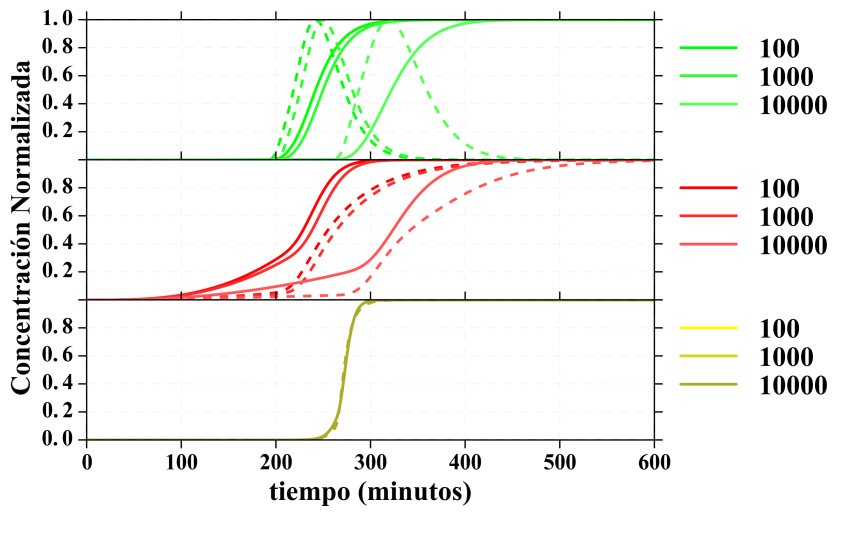
\includegraphics[width=0.9\textwidth]{./img/Cap3/SweepAll.png}
    \caption{Concentraciones normalizadas correspondientes a cada tipo de sensor sin clivar en función del tiempo para distintas concentraciones iniciales. Las concentraciones iniciales de cada sensor sin clivar se mantuvieron iguales entre sí en cada simulación.}
    \label{fig:sweepcc}
\end{figure}

%Por otro lado, es importante recalcar que cada sensor transfectado se hallaba en un plásmido distinto. Esto implica que no necesariamente se transfectaban los tres sensores simultáneamente a la misma célula, e incluso puede que más de una copia de alguno se haya transfectado a ésta.
Las concentraciones iniciales de cada sensor no son necesariamente iguales, pudiendo producir estancamientos en alguno de los pasos de la cascada de señalización. Los efectos de tener elevadas concentraciones iniciales de algún sensor puede implicar mayores diferencias temporales entre la activación de algunas caspasas y se explica mediante fenómenos de secuestro de enzima (caspasa) por el sustrato (sensor). Estos fenómenos de diferencias en concentraciones iniciales se traducen en retrasos temporales entre los tiempos en que se cliva cierto porcentaje del sensor. Consideremos, por ejemplo, lo que sucede con los momentos en que se cliva el 10$\%$ o el 50$\%$ del sensor. 

\begin{figure}
    \centering
    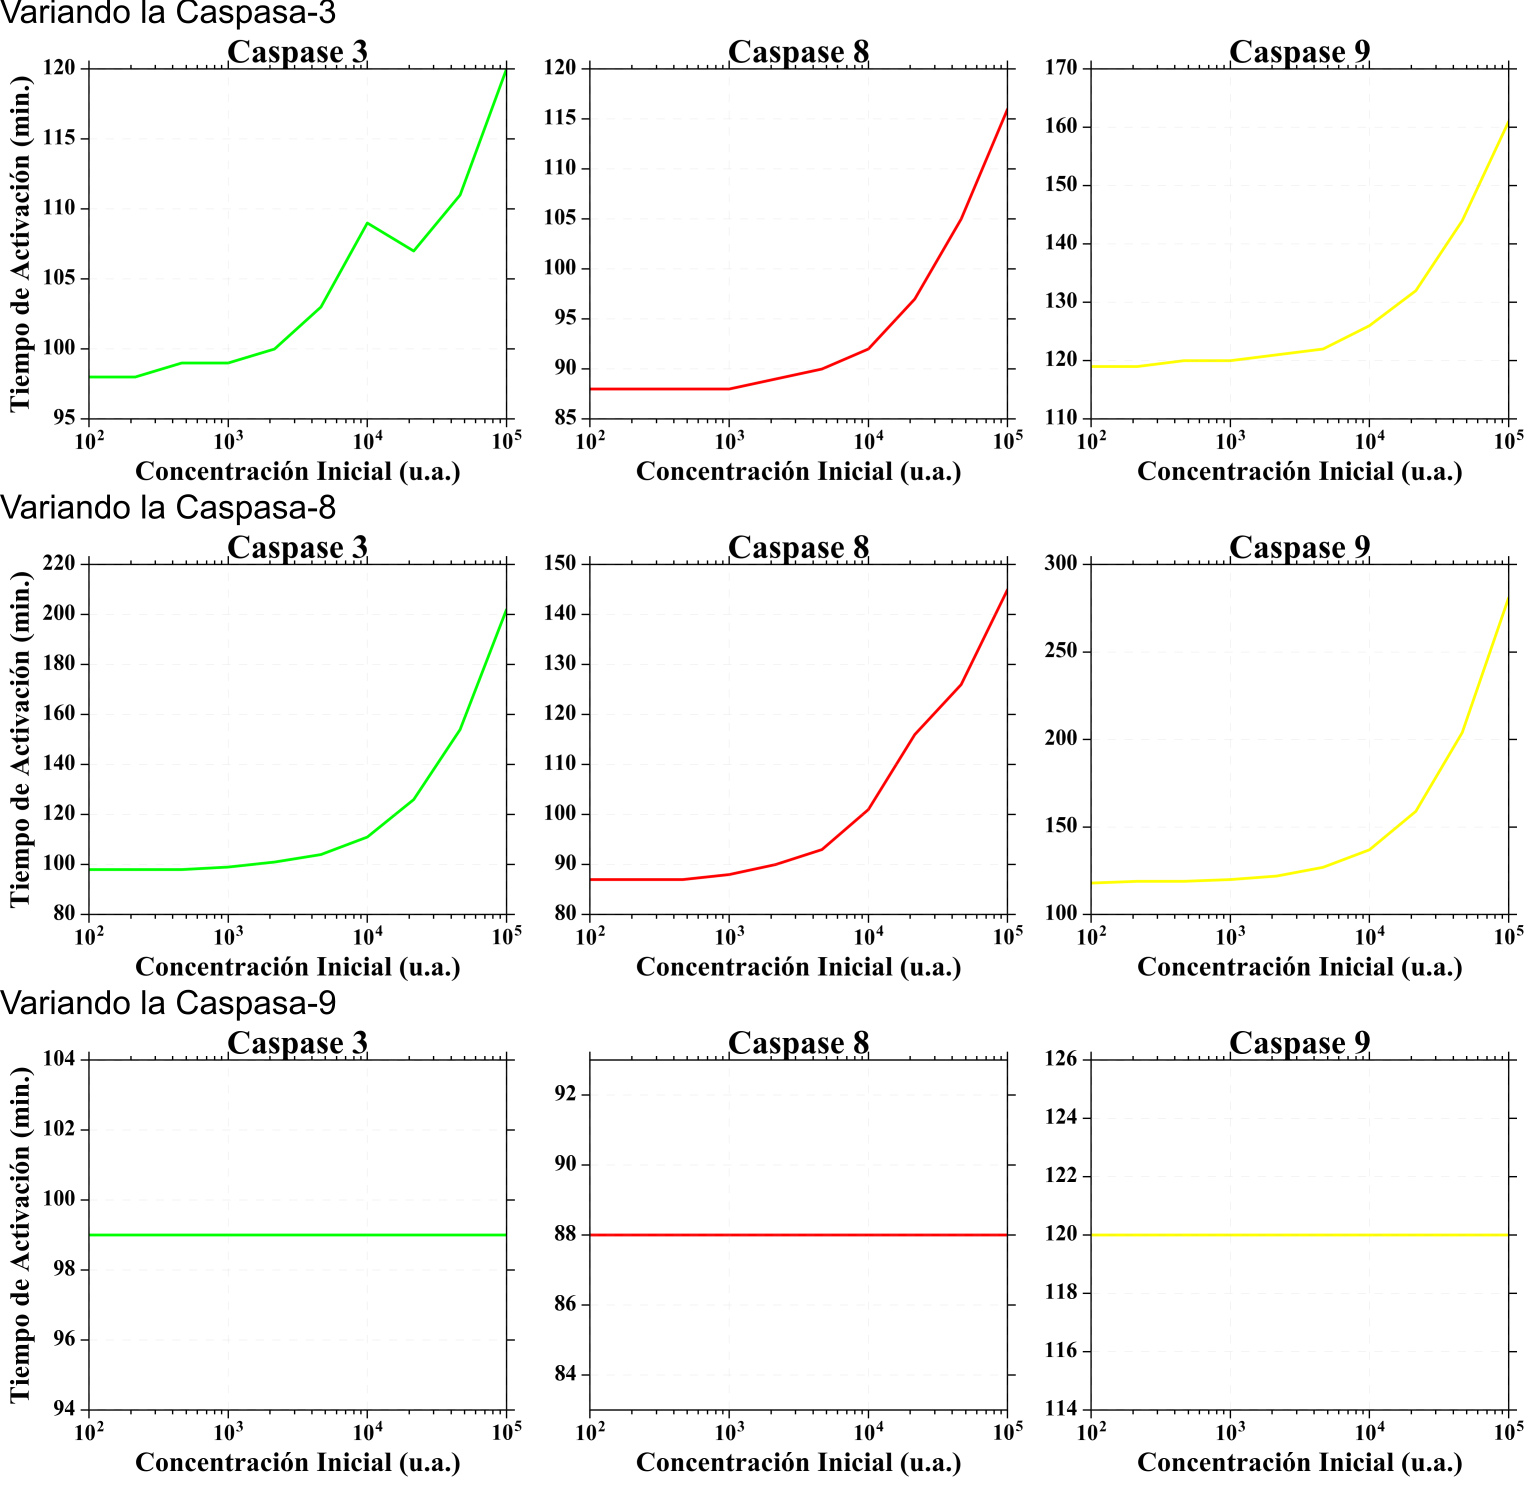
\includegraphics[width=0.9\textwidth]{./img/Cap3/Varcp10.png}
    \caption{Variación del momento en que se alcanza el clivaje de 10$\%$ de los biosensores utilizados. Se presentan en las distintas filas las simulaciones en que se variaba la concentración inicial de un único biosensor.}
    \label{fig:varcp10}
\end{figure}

En las figuras \ref{fig:varcp10} y \ref{fig:varcp50} se presentan gráficos del tiempo de activación definido como el momento en que se cliva el 10$\%$ o el 50$\%$ de sensor, respectivamente, según la concentración inicial de sensor utilizada. Este tipo de análisis provee información valiosa sobre el sistema y como se interrelacionan sus elementos. Tomemos por ejemplo la segunda fila de imágenes de la figura \ref{fig:varcp10} que corresponde a estudiar el momento en que se cliva 10$\%$ del sensor y se varia la concentración inicial del biosensor para caspasa-8. Se observa que la variación en el tiempo de activación de las tres caspasas. Esto se debe a que la caspasa-8, iniciadora en la vía extrínseca se encuentra menos alocada a activar la caspasa-3 y la vía intrínseca ya que se ve secuestrada por el biosensor. Aunque este tipo de análisis exhaustivo puede aplicarse a muchas simulaciones distintas, solo se presentarán las más relevantes para el trabajo realizado. Se debe destacar que la velocidad de la caspasa-9 es al menos un orden mayor que las otras, por esta razón no se ve afectada por fenómenos de secuestro.

\begin{figure}
    \centering
    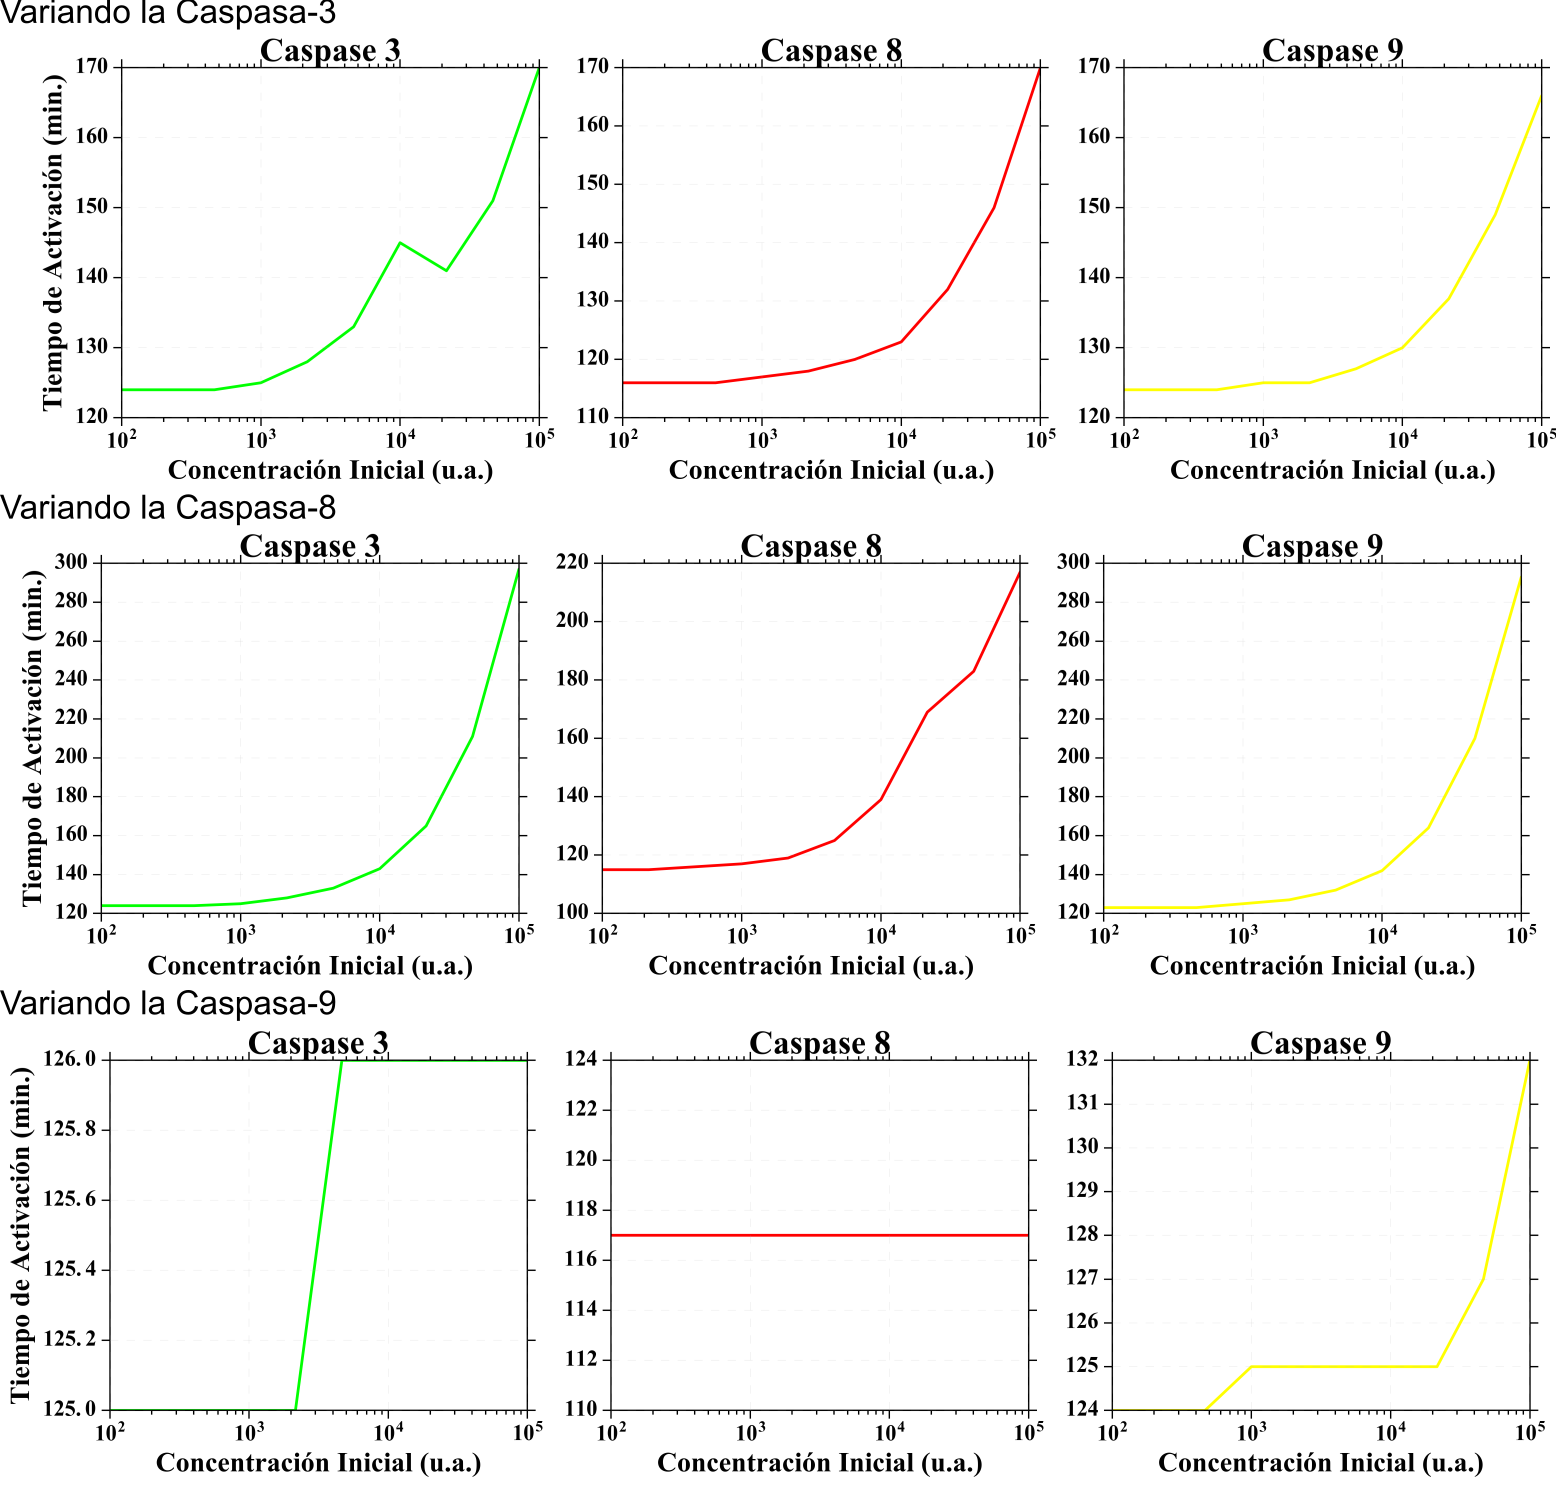
\includegraphics[width=0.9\textwidth]{./img/Cap3/Varcp50.png}
    \caption{Variación del momento en que se alcanza el clivaje de 50$\%$ de los biosensores utilizados. Se presentan en las distintas filas las simulaciones en que se variaba la concentración inicial de un único biosensor.}
    \label{fig:varcp50}
\end{figure}

Es importante destacar que las diferentes concentraciones de biosensor tienen doble efecto sobre el análisis que queremos realizar en el sistema. En primer lugar, cantidades elevadas de biosensor alteran la dinámica de la red produciendo resultados poco fieles a la dinámica fisiológica de este. Por otro lado, concentraciones bajas de biosensor implica que el clivaje total del sensor ocurrirá rápidamente y no será posible apreciar la dinámica de éste a tiempos largos.

%%%%%%%%%%%%%%%%%%%
\subsection{Degradación de la Caspasa-3}

A continuación, se estudiaron los efectos de incluir la degradación de la caspasa-3 en el modelo matemático. En primer lugar, se observó que si la caspasa-3 comienza a ser degradada inmediatamente después de ser activada, esta ejerce su función de clivaje durante una ventana temporal acotada. Esto se refleja, en parte, en que no todo el sensor disponible es clivado por la caspasa-3, como puede observarse en la imagen \ref{fig:deg_casp3}. Puede apreciarse que la proporción de caspasa activa comienza y termina en cero.

\begin{figure}
    \centering
    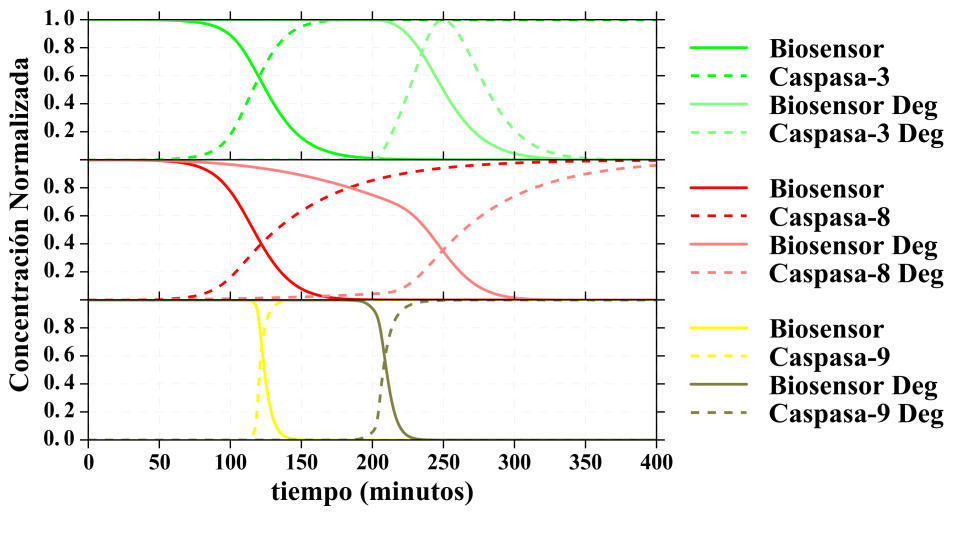
\includegraphics[width=0.9\textwidth]{./img/Cap3/ConSinDeg.png}
    \caption{Se presentan gráficos superpuestos de las curvas correspondientes al sensor sin clivar y la caspasa activa para las simulaciones en que se activaba la degradación de la caspasa-3 (Deg) y las que no.}
    \label{fig:deg_casp3}
\end{figure}

Por otro lado, se deben recalcar los efectos que la degradación o ausencia de degradación de la caspasa-3 tiene sobre el orden de activación de las caspasas. Resulta intuitivo que activar la degradación producirá no solo un retraso en su activación, sino que también se verá disminuida la actividad del lazo de retroalimentación con la caspasa-8, demorando a su vez la activación de esta otra caspasa. Estos efectos pueden deducirse de la cascada de señalización de caspasas.


%%%%%%%%%%%%%%%%%%%
\subsection{Lazo de Retroalimentación de la Caspasa-6}

Como se aprecia en la figura \ref{fig:ModeloCompleto}, el rol de la caspasa-6 es el de servir de medio de retroalimentación positiva entre la caspasa-3 activa y la procaspasa-8. En el trabajo presentado por \textit{Sorger et al.}, este mecanismo de retroalimentación es desactivado con el único fin de confeccionar una imagen. De todas formas, se decidió estudiar sus efectos en el modelo adaptado.

\begin{figure}
    \centering
    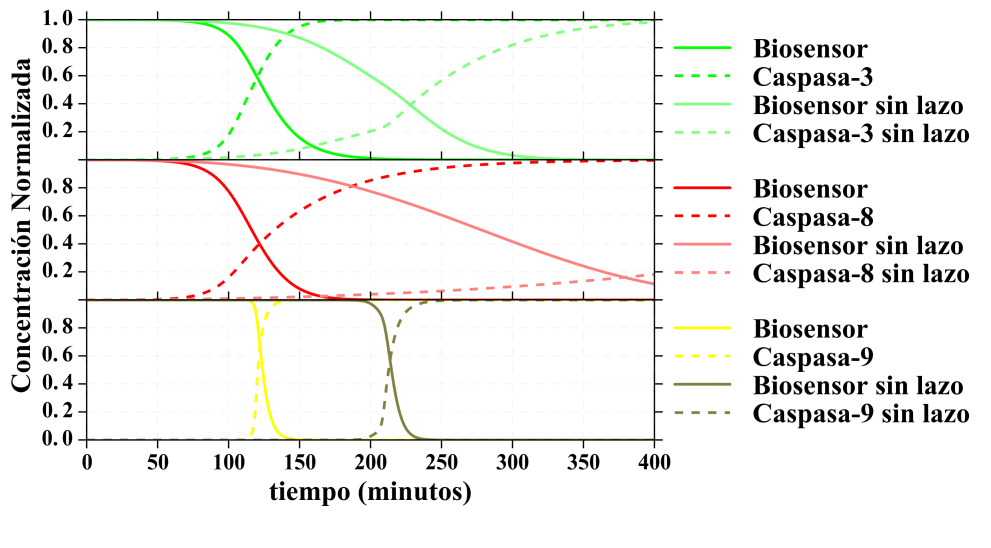
\includegraphics[width=0.9\textwidth]{./img/Cap3/ConSinC6.png}
    \caption{Se presentan gráficos superpuestos de las curvas correspondientes al sensor sin clivar y la caspasa activa para las simulaciones en que se activaba el lazo de retroalimentación de la caspasa-6 y los que no (sin lazo).}
    \label{fig:casp6}
\end{figure}

En la figura \ref{fig:casp6} se muestran los efectos que tiene el lazo de retroalimentación en estudio. Como es de esperarse, su papel principal es el de fomentar la activación de caspasa-8 una vez que se encuentra activa la caspasa-3. Su inactivación se ve reflejada en el incremento de la diferencia temporal que hay entre las activaciones de la caspasa-3 y -8.


%%%%%%%%%%%%%%%%%%%%%%%%%%%%%%%%%%%%%%%%%%%%%%%%%%%
\section{Estado de la Caspasa Inferido a Partir del Estado del Sensor}

Una vez adaptado el modelo matemático para incluir el comportamiento de los sensores, se analizaron que parámetros son útiles para recuperar información valiosa sobre el estado de este.
%Haciendo uso del método de ajuste presentado en el capítulo \ref{cap:microscopia}, que nos permite encontrar la proporción de fluoróforo en estado monomérico a partir de la curva de anisotropía del sistema, podemos implementar métodos para inferir el estado de la caspasa en estudio.

Conociendo la proporción de sensor en un estado clivado podemos estimar la cantidad de complejo caspasa:sensor calculando su derivada y normalizando. Esto se deduce utilizando la ecuación análoga a la ecuación \ref{eq:cin_prod} que relaciona la velocidad de formación de producto, o sensor clivado en este caso, con la concentración de complejo. Una posible interpretación de esta variable, $\Delta m$ es que representa la cantidad de caspasa que se encuentra clivando sensor en cada instante, es decir, ofrece una lectura sobre la actividad caspasa. %Esta claro que depende de la existencia de sensor sin clivar para poder ofrecer alguna lectura.

De todas formas, debe tenerse cuidado con su interpretación ya que solo funciona si la concentración del sensor en la célula se encuentra dentro de un rango dinámico comparable a otras especies de la célula. En particular, si hay poco sensor dentro de la célula, se observará una actividad máxima muy temprana que dura unos pocos minutos. Mientras que si la concentración del sensor es demasiado alta, la red de caspasas se verá muy perturbada por el sensor y el sistema presentará un comportamiento alejado de la realidad.

Debido a las constantes de reacción involucradas en las reacciones de clivaje del sensor, el modelo predice que las concentraciones de complejo caspasa:sensor son al menos cuatro ordenes más chicas que las concentraciones de sensor. A esto debe sumarse que por conservación de la cantidad de biosensor, $s+c+p$ es un valor constante, y si despreciamos $c$, podemos obtener el valor de $s$ a partir de $-p$.

A continuación, teniendo en cuenta el efecto que tiene la cantidad de sensor inicial sobre el parámetro relacionado con la actividad de la caspasa, se decidió dividir la derivada temporal de la proporción de sensor clivado por la concentración de sensor sin clivar. Este parámetro, que llamaremos $\Delta m/d$ normalizado nos reporta de forma robusta la proporción de caspasa activa. Puede apreciarse en la figura \ref{fig:Deltams} la superposición entre las especies normalizadas de complejo caspasa:sensor y caspasa activa con sus reporteros $\Delta m$ y $\Delta m/d$, respectivamente.

\begin{figure}
    \centering
    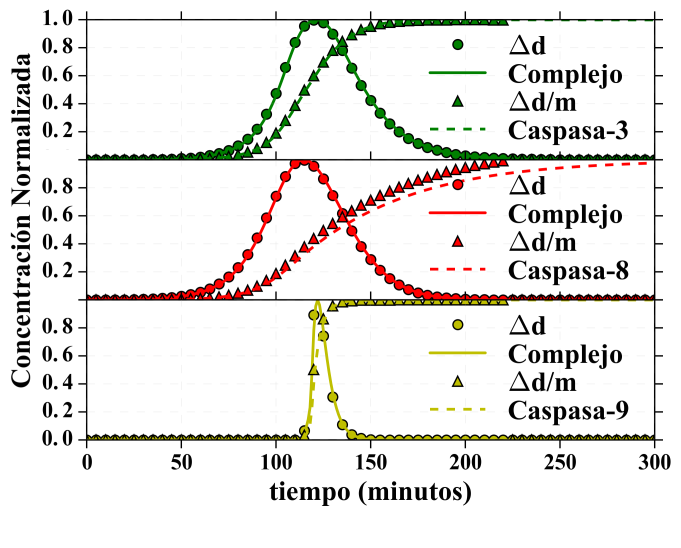
\includegraphics[width=0.9\textwidth]{./img/Cap3/Metodo.png}
    \caption{Gráfico de proporción de caspasa activa y caspasa en complejo con biosensor en función del tiempo y superpuesto con $\Delta m$ y $\Delta m/d$. Se puede apreciar la elevada similitud entre el complejo caspasa:sensor y $\Delta m$, así como también entre la caspasa activa y $\Delta m/d$.}
    \label{fig:Deltams}
\end{figure}

Existen diversas consideraciones que deben tenerse en cuenta para analizar este parámetro. Para comprender mejor de donde surge este parámetro, podemos apreciar que antes de que se active la caspasa, la cantidad de sensor sin clivar es máxima, mientras que como no hay variaciones en la proporción de sensor clivado el valor de $\Delta m/d$ nos reporta que la proporción de caspasa activa es nula. Si nos concentramos en el otro extremo, la cantidad de sensor sin clivar tiende a cero, al igual que la variación de sensor clivado. Si el numerador y denominador tienden a 0, pero el denominador lo hace más rápido, entonces al normalizar observaremos que la proporción de caspasa activa es máxima, y se corresponde con el estado del sistema.

Para comprender que sucede durante la transición será necesario considerar despreciable la concentración total de complejo caspasa:sensor frente a la concentración total de enzima y sensor libre. Dado que el modelo matemático se condice con esta aseveración, podemos utilizar la ecuación \ref{eq:cin_sens} para mostrar que despreciando el valor de $c$, llegamos a que

\begin{equation}
    \frac{ds}{dt} = - k_+ se,
\end{equation}

\noindent de donde se deduce que dividir la variación de sensor en estado dimérico por su concentración es proporcional a la cantidad de enzima activa. De esta forma, es válido utilizar $\Delta m/d$ (ó $\Delta p/s$) normalizado para estimar la proporción de caspasa activa. También deben tenerse los mismos recaudos que se tuvieron para $\Delta m$ si se utilizan concentraciones iniciales de sensor muy altas o muy bajas.

Finalmente, se repitieron los cálculos para distintas simulaciones donde se utilizaron diferentes concentraciones iniciales para cada sensor. Se recuperaron adecuadamente las curvas normalizadas de complejo caspasa:sensor así como la proporción de caspasa activa para todas las simulaciones, excepto cuando las concentraciones utilizadas eran exageradas. De esta forma, se deduce que dentro del rango de concentraciones posibles para el sensor, este estudio reporta adecuadamente la proporción de caspasa activa.